%! TEX root = 'main.tex'
\section{Implementation and Experiment}
\label{sec:implant-implementation}


This section provides the implementation details and discusses the issues that we encountered during the development. 
%We also give some experiments to prepare for attacks in different scenarios, which are not used in the current prototype.


\textbf{\texttt{Read/Write Memory.}} We briefly introduced the JTAG protocol in the background (~\autoref{sec:implant-background}) earlier. Our driver sends instructions to the IR and reads the returned result according to the JTAG state machine. Nevertheless, we need to know how to operate ARM's CoreSight components for this particular hardware backdoor prototype. We choose the JTAG interface instead of SW (Serial Wire), so the corresponding debug port is JTAG-DP or SWJ-DP, as shown in~\autoref{fig:dap}.

\begin{center}
	\begin{table}
		\small
		%\begin{tabular}{p{1.6cm}  p{1.6cm}  p{4cm}} 
		\begin{tabular}{l l l l} 
			\hline
			\makecell{IR \\ value} & \makecell{JTAG-DP \\ Register} & \makecell{DR \\ width} & Description  \\ 
			\hline
			%\multicolumn{3}{l}{\textbf{Memory} (0x00000000 - 0x22200000)}  \\
			%\hline
			b1000 & ABORT & 35 & JTAG-DP Abort Register \\
			\hline
			b1010 & DPACC & 35 & JTAG DP Access Register \\
			\hline
			b1011 & APACC & 35 & JTAG AP Access Register\\
			\hline
			b1110 & IDCODE & 32 & JTAG Device ID Code Register \\
			\hline
			b1111 & BYPASS & 1  & JTAG Bypass Register \\
			\hline
		\end{tabular}
		\caption{DPACC is used for Debug Port (DP) accesses. APACC is used for Access Port (AP) accesses, and it can access a register of a debug component of the system to which the interface is connected.}
		\label{tab:jtag-dp}
	\end{table}
\end{center}



Through DPACC and APACC registers, the debugger can access resources provided by other access ports (AP).  As mentioned earlier, an access port provides the interface between the debug port interface and one or more debug components present within the system. There are two kinds of access ports: Memory Access Ports (MEM-AP) and JTAG Access Ports (JTAG-AP), and MEM-AP is designed for connects to memory bus system with address and data controls.  Since our backdoor wants to access memory and GPIO, we need to access either AHB-AP or the MEM-AP, which handled the differences between the underlying bus.



\begin{figure}[ht]
	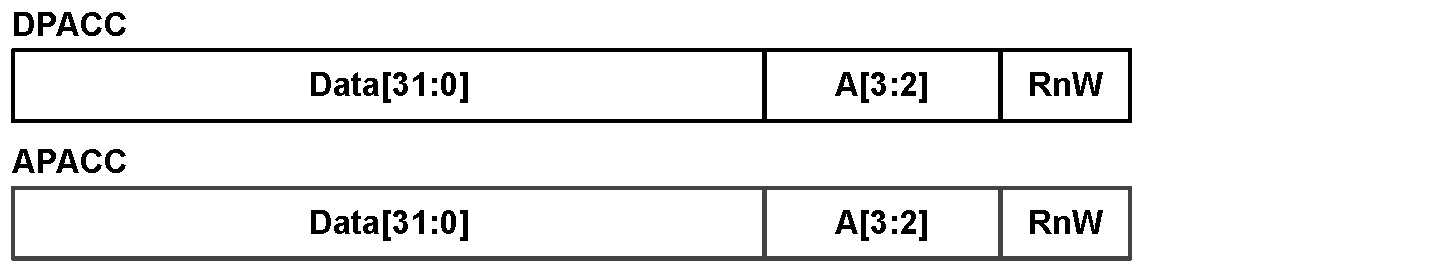
\includegraphics[width=0.47\textwidth]{figures/dpapacc}
	\centering
	\caption{Both of the two registers are 35 bits long and can be scanned in/out through the JTAG protocol with IR instruction b1010 and b1010, respectively. RnW takes one bit, and zero indicates a write. A[3:2] selects the register within a bank.}
	\label{fig:dpapacc}
\end{figure}


~\autoref{fig:dpapacc} shows that both DPACC and APACC have the same structure, and they can be scan in/out through the JTAG state machine with the specific IR instruction value. The lowest bit indicates whether to read or write DP/AP, where zero means write.

 According to ARM Debug Interface Architecture Specification v5.0 to v5.2, every bank has four registers, and A[3:2], the two bits are used to select the register from the bank. The DP only has one bank, and the MEM-AP has 16 banks, as listed in~\autoref{tab:dpreg} and ~\autoref{tab:memapreg}, respectively. To select the AP's bank, we also need to write the bank address into the DP's SELECT register.




\begin{center}
	\begin{table}
		\small
		%\begin{tabular}{p{1.6cm}  p{1.6cm}  p{4cm}} 
		\begin{tabular}{l l l} 
			\hline
			Offset & Register &  Description  \\ 
			\hline
			%\multicolumn{3}{l}{\textbf{Memory} (0x00000000 - 0x22200000)}  \\
			%\hline
			0x00 & & Reserved \\
			\hline
			0x04 & CTRL/STAT & Control and State Register \\
			\hline
			0x08 & SELECT & AP Select \\
			\hline
			0x0C & RDBUFF & Read Buffer\\
			\hline
		\end{tabular}
		\caption{Debug Port registers. Debug Port only has one bank, a total of four registers, which can be specified by A[3:2] of the DPACC register. }
		\label{tab:dpreg}
	\end{table}
\end{center}

\begin{center}
	\begin{table}
		\small
		%\begin{tabular}{p{1.6cm}  p{1.6cm}  p{4cm}} 
		\begin{tabular}{l l l} 
			\hline
			Offset & Register &  Description  \\ 
			\hline
			%\multicolumn{3}{l}{\textbf{Memory} (0x00000000 - 0x22200000)}  \\
			%\hline
			0x00 & CSW & Control/Status Word register \\
			\hline
			0x04 & TAR & Transfer Address Register \\
			\hline
			0x08 & & Reserved \\
			\hline
			0x0C & DRW & Data Read/Write register\\
			\hline
			... & & \\
			\hline
			0xFC & IDR & Data Identification register\\
			\hline
		\end{tabular}
		\caption{Part of Memory Access Port (MEM-AP) registers. MEM-AP has 16 banks, and each bank has four registers, which can be specified by A[3:2] of the APACC register. The bank needs to be specified by the DP:SELECT register.}
		\label{tab:memapreg}
	\end{table}
\end{center}





To read and write memory, we need to use the internal registers provided by the MEM-AP. Specifically, we need to sue CSW, TAR, DRW, and others. Since these registers are in the MEM-AP's bank 0, we must first use DPACC to select it. Take writing memory as an example. Next, we need to write the destination address to TAR and then write the value to DRW. ~\autoref{fig:memapwrite} shows a pseudo-code for writing memory.


\begin{figure}[ht]
	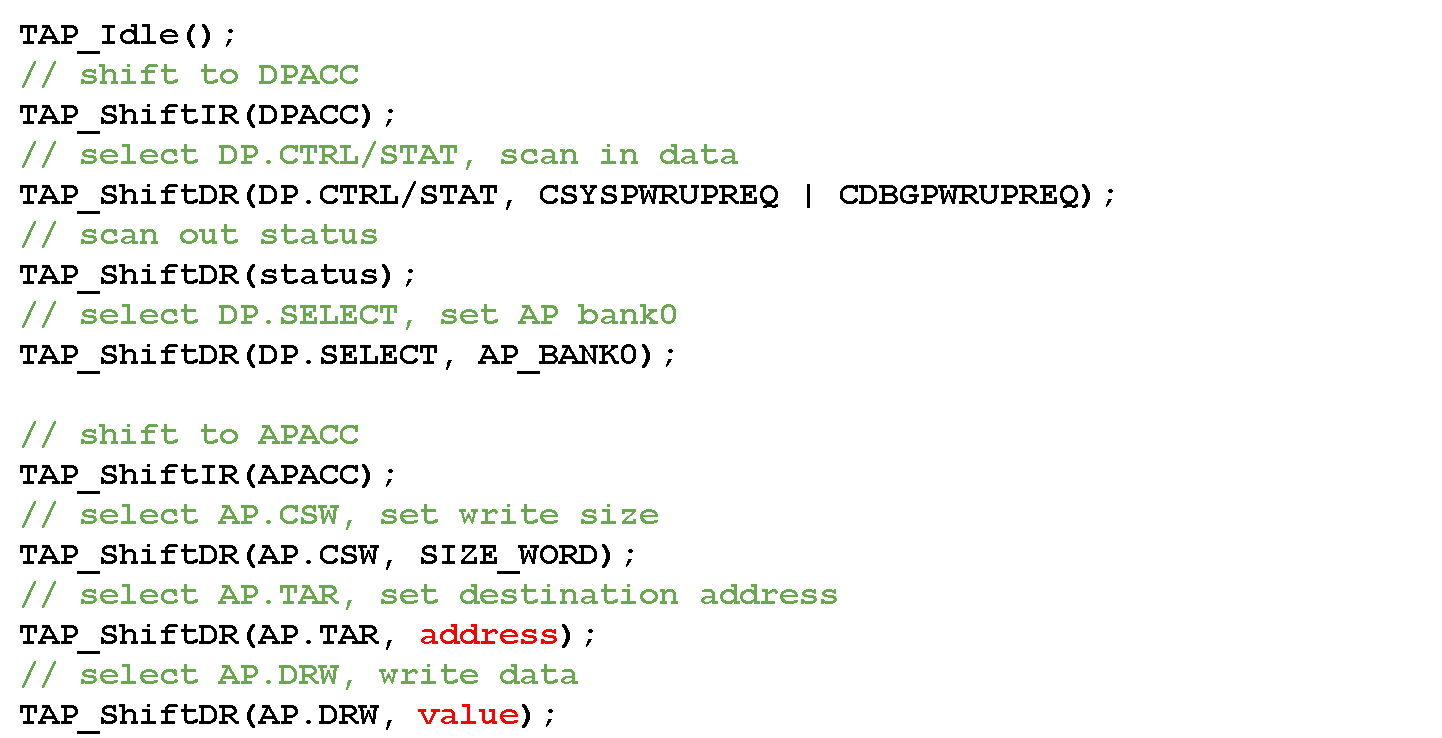
\includegraphics[width=0.47\textwidth]{figures/memapwrite2}
	\centering
	\caption{Pseudo-code for memory writing through MEM-AP. Notice, CSW, TAR and DRW are all in the bank zero. However, the bank is specified in the DP.SELECT instead of a register in AP.}
	\label{fig:memapwrite}
\end{figure}




\textbf{\texttt{Send/Receive SMS Message.}} SIM800C provides a serial port as the interface to receive AT commands. When \name is started, we use the AT+CMGF command to set the GSM chip in SMS Text Mode. Then we use the AT+CNMI command to set how to notify when new messages come. After that, the Teensy board keeps checking the serial port for new messages every second. If there is one, read the content and parse if it is a pre-defined attack command.

To send out a message, use the AT+CMGS command to set the destination phone number and then send the text message to the serial port. 


\textbf{\texttt{Intercepting SPI Data.}} As mentioned earlier, we can directly control the power switch chips to change the output or modify the transmission data by intercepting the bus on the circuit board, mainly low-speed buses such as SPI. For example, if we change a pin from zero to one, we need to connect it to the high voltage (3.3v) power supply to override the original signal. Similarly, we ground it to force it a zero. 
However, these operations need to consider the IC's interface.

The pins of the SPI flash chip use a push-pull configuration rather than an open drain. The output pins can actively create their own logical high and low states instead of relying on pull-up resistors to generate a default state. However, in this way, we must add an appropriate current-limiting resistor when forcing the signal to the ground or power supply to avoid short circuits.

For the SPI protocol, we modify the MOSI data line according to the SCLK clock signal, and we use FPGA to implement this circuit. In each clock cycle of SPI, we first read the data transmitted on the MOSI and store it into a shift register. When finding the target pattern, we modify the following data. To meet the setup time required for the SPI data line, we choose to make the circuits work on the clock's falling edge, given that the SPI works on the rising edge.
